\section{Foundry} 
\label{sec:approach}

%\eb{Will resume working from here.}
%\todo{Paulo veja esta frase abaixo. Ao meu ver ela não esta correta.}

Based on software transplantation idea, \FOUNDRY treats \emph{product base} and \emph{over-organs} (representing features) as product line assets. 
A product base is a host that contains all features that will be shared among the products. 
An over-organ, in turn, is a completely functional and reusable portion of code extracted from a donor system that conservatively over-approximates the target organ~\cite{Barr2015}. An over-organ can be specialized to became an organ that preserves the original behavior of the feature in a different host codebase~\cite{Barr2015}.

Conceptually, in \FOUNDRY, while the product base provides commonalities (i.e., common features) to the target product line, the variability (i.e., variant features) are provided by the transplantation process, as illustrated in \Cref{fig:product_for_transplantation}. This idea opens new ways for SPLE area by automated construction of different products by transplanting multiple organs into a product base. 

\begin{figure}[t]
	\centering 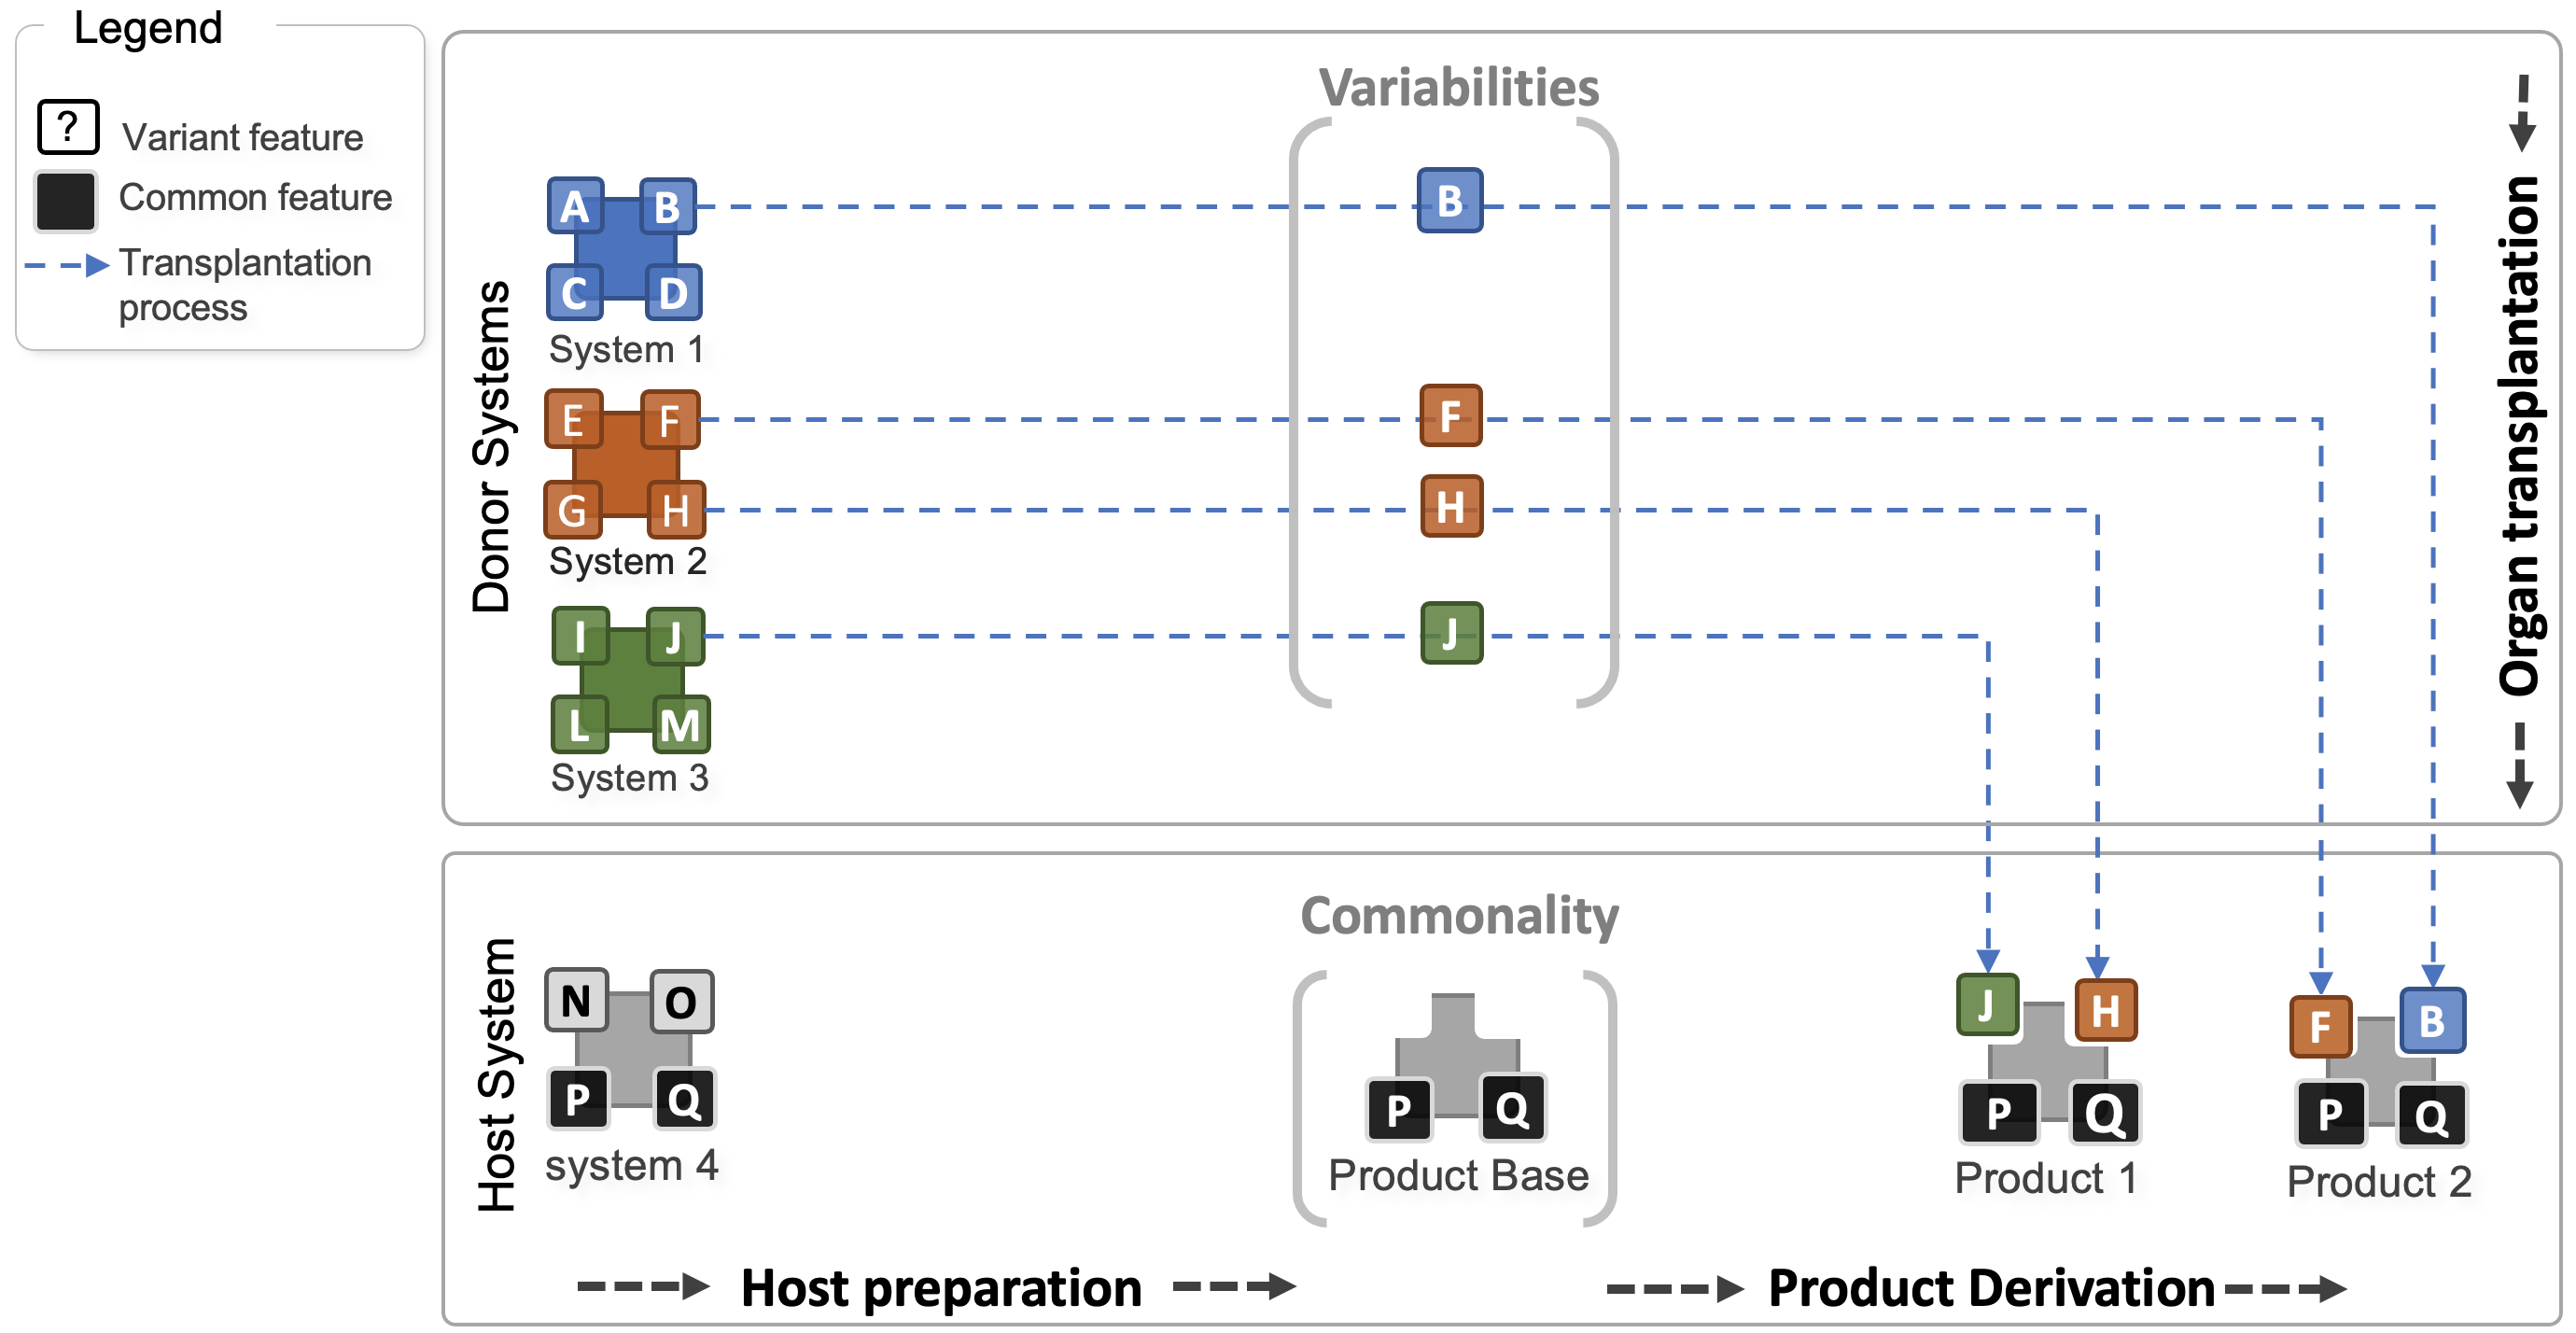
\includegraphics[width=\textwidth]{images/product_for_transplantation7.png}
	\centering 
	\caption{An overview of how new products are derived from a product line based on ST.}
	\label{fig:product_for_transplantation}
\end{figure} 

%\todo{to be removed: It is important to note that \FOUNDRY offers two ways of creating products. One can store over-organs into a given platform of core assets (as in traditional SPL, where a selection of features is enabled). Alternatively, we can create a product by directly extracting and transplanting an organ from a donor into a product base, even if the over-organ is not present in our transplantation platform.}

It is important to note that \FOUNDRY offers two ways of creating products by transplanting organs from a pre-established/created \emph{transplantation platform}, a repository of transplantation assets, or by directly extracting and transplanting an organ from a donor into a product base, even if the over-organ is not present in the transplantation platform. The two ways can also be combined to create specialized products.

In the rest of this section, we overview \FOUNDRY's workflow, describing how it applies software transplantation idea to reengineering of product lines from existing systems. \FOUNDRY is independent of the programming language, and supports SPL's \emph{domain engineering} and \emph{application engineering}~\cite{Clements2001} processes at the code level.

\subsection{Domain Engineering}

In SPL's lifecycle the domain engineering corresponds to the process of establishing a reusable platform of core assets~\cite{Clements2001}. The process defines what will be shared among the products derived from it, i.e., commonalities. It also specifies the possible variations expressed as artefacts, that will enable the customization of product line applications, i.e., products.

In \FOUNDRY, domain engineering corresponds to the process of establishing a product line composed of a product base and a set of reusable over-organs extracted, both stored in the transplantation platform. \Cref{fig:foundry_dom} illustrates the stages of the domain engineering process. 

As in medicine, \FOUNDRY has a \emph{preoperative} stage where donors and the host are prepared for the transplantation process and a \emph{postoperative} stage where we evaluate if the transplantation was successful (\Cref{sec:application_eng} for more details on the postoperative stage). The preoperative stage defines pre-transplantation tasks, responsible for the variability analysis process, the organ's test suite, donor and host preparation.

\begin{figure}[t]
	\centering  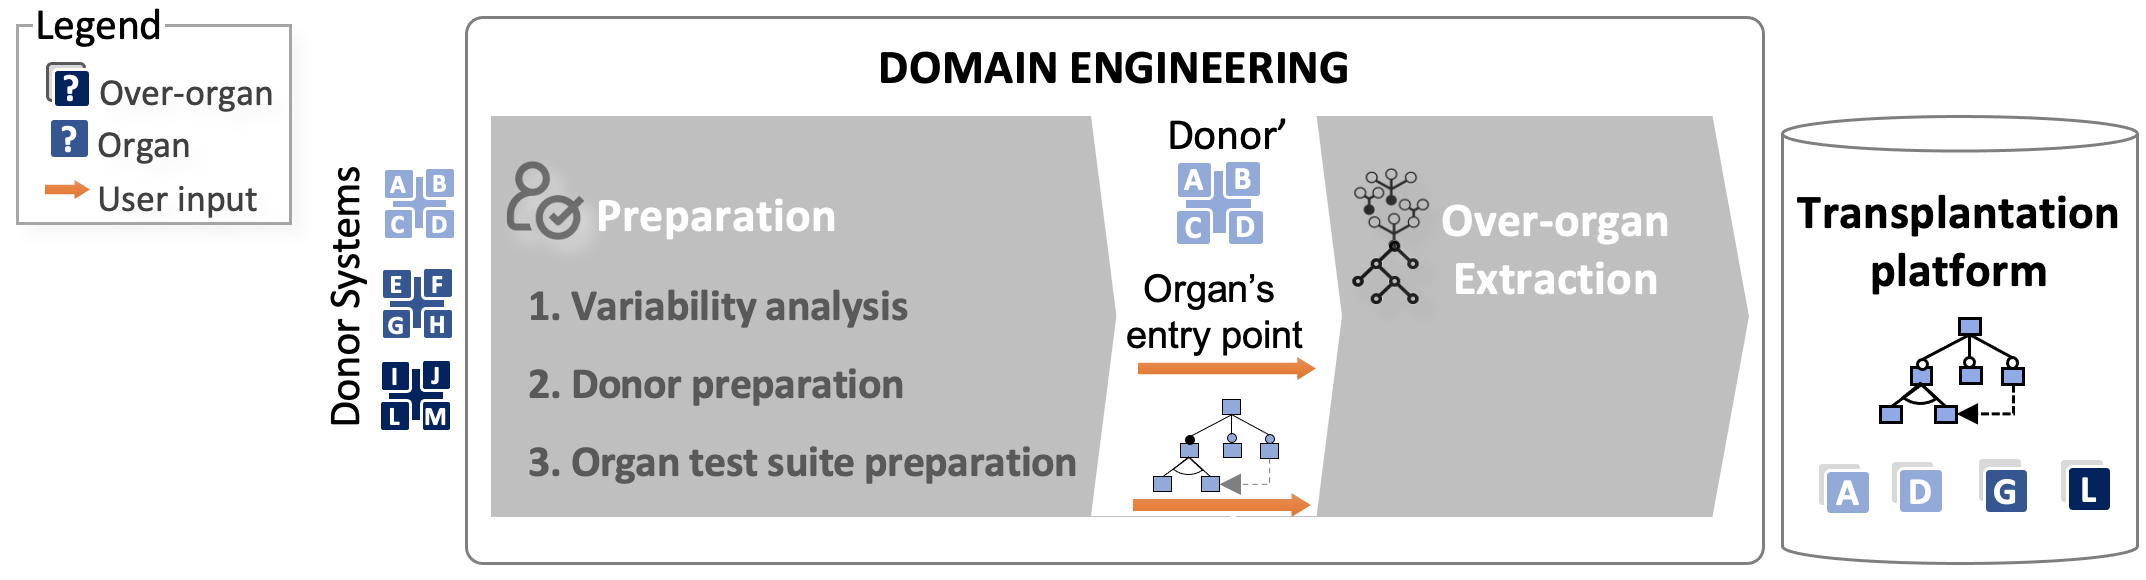
\includegraphics[width=\linewidth]{images/FOUNDRY_DOM6.png}
	\centering \caption{Domain engineering process supported by FOUNDRY. \textit{Four over-organs (A, D, G, L) are extracted from three donor systems and kept in the transplantation platform, with product base consisting of 2 features shared across all products (P and Q).} }
	\label{fig:foundry_dom}
\end{figure} 

%\subsection{Preoperative stage}


\textbf{Variability Analysis.} The preoperative stage starts with a variability analysis process to discover features in existing products with the potential to create the target product line. This process aims to create a variability model to express the valid combinations of features among the donor systems from which they will be extracted.  

A variability model can be represented by using a feature model~\cite{Kang1990}. We augmented the traditional feature model representation to incorporate software transplantation inputs required to manipulate and maintain the over-organs in the product line. Each over-organ representation in the feature model is annotated with its corresponding entry point in the donor codebase. 
An organ's entry point is a function in the donor system that belongs to the organ, defines an execution environment expected for its initialization, and provides access to the organ's test suite~\cite{Barr2015}. To determine the organ’s entry point, the SPL engineer needs to provide the name of the function implemented in the donor codebase.

\textbf{Donor Preparation.} This task in the preoperative process consists of cleaning up of donor codebases.  
These can contain some code that will never be used in the target products.
For example, codebases written in C, in general, have code fragments guarded by \#ifdef C-preprocessor directives~\cite{Tartler2011})  commonly used to control code extensions related to features. Although useful for the donor program, such code, if transplanted as part of the target organ, will generate dead code ~\cite{Tartler2011} that will never be executed in any transplanted product.  

Previous work~\cite{Barr2015} with focus on transplantation of a single feature did not concern with donor clean-up. 
However, even when transplanting a single organ, dead code, if not removed apriori, can lead to unnessasary bloat and lower efficiency of the over-organ adaptation process (\Cref{sec:application_eng}). 
In \FOUNDRY, the donor clean-up can be performed in a manual or automated way. During the process the source code structure of the program needs to be preserved (indentation, spacing, number formats, etc.), to prevent future bugs. 

\textbf{Organ Test Suite Preparation.} For product derivation, an SPL engineer must supply test suites, called \emph{ice-box tests}~\cite{Barr2015}. They are used to guide genetic programming in the over-organ adaptation process to create an organ that is fully executable when implanted in the product base (see \Cref{sec:organ_reduction}). 
Ice-box tests can be easily implemented as proposed by~\cite{Barr2015} and integrated into the transplantation platform to be used for new transplantations of the target organ. 
These can be quick to develop, using existing test generation tools, or even adapted from donor’s unit tests, when available.

Even though the preparation process may require manual effort for identifying features of interest,  localising and removing  dead code from the donor and preparing all test suites for the organ, it can be amortised across multiple transplantations and reuse of a single over-organ.

\textbf{Host preparation.} The SPL engineer has to select a product base. It is an existing system which already provides a set of solutions (features) so close to the target products that it can be used as a baseline for the assembly of products. For example, a text editing program could provide a baseline for new programs for text translation,  presentation or rendering, since they could have a considerable number of common features between them.

In case it is necessary, the product base can be reduced to its basic form, keeping only mandatory or features relevant to the target product line. The reduction process consists of removal of all code that implements all features which will not be required to create the target products. In a removal scenario, an additional attention is necessary to find and remove all portions of code that implement each unwanted feature without compromising the product base.

A product base, once reduced, can be used multiple times as a base for new products. Although its preparation may require considerable effort for localising and removing all unnecessary code, it can be compensated with the benefits achieved through using the product base as a baseline to build other products belonging to the same or similar domain.

\textbf{Over-organ Extraction.} Once the donor is prepared, it is possible to start the over-organ extraction process. In this stage,  all source code related to the organ to be transplanted, that implements the target feature, must be identified and extracted. 

Conceptually, an over-organ is composed of an organ and its vein, in keeping with the transplantation analogy~\cite{Barr2015}. While the organ implements the functionality we wish to transplant, the vein is a path from the donor entry that builds and initializes an execution environment for the organ~\cite{Barr2015}. Thus, all the code belonging to the organ and its vein must be captured in the extraction process.

In practice, organs can consist of several lines, one or more classes, as long as they fully implement a specific functionality~\cite{Wang2018}. We consider an organ to be a functional implementation of a feature of interest to an emergent product line. 
This makes the code extracting process a challenging task since it also involves identifying all code elements for the organ to be kept functional even out of the donor's environment.
The extraction of a target over-organ can thus involve a considerable amount of code at different levels of granularity, from moving required files and libraries to entire functions and individual statements, both potentially not confined to a single class, file or library~\cite{Wang2018}. For instance, the feature $\texttt{FEAT\_DIFF}$ implemented in VIM has more than 5k LOCs scattered across 33 of its 166 source files. 
Previous work extracted features from a single file~\cite{Barr2015}.

Here we have four challenges that need special attention. 
First challenge concerns the integrity of the extraction when the extracted code appears in several files, issue also identified by Wang et al.~\cite{Wang2018}. 
In this case, the extracted organ also needs to preserve the original multi-file structure. 
Otherwise, it may be even more difficult to keep it functioning outside of  the donor's environment or to propagate eventual changes to the desirded feature (bug fixes, enhancements, etc.).
Second, defects might be introduced due to code redundancy stemming from multiple organ transplantations. 
Multiple organs can use the same code, creating code duplication and possible errors, if not handled correctly.
Third, an organ's vein can contain a large amount of code, especially when the host and the donor have very different structures. 
This requires extensive modification during the adaptation process. 
According to Barr et al.~\cite{Barr2015},  inlined function calls constitute the second largest number of code lines transplanted. 
Fourth challenge is that an extracted over-organ may itself contain multiple smaller features, which its functionality depends on.
For example, a $\texttt{spell\_checker}$ feature might depend on a memory-resident database feature. 
Thus, the extraction process has to implicitly learn feature's dependencies, by including them in its over-organ. 
Such issues, if not solved, make impracticable the generation and maintenance of product lines using the software transplantation approach. 

To solve all additional challenges highlighted above, we have evolved the organ extraction process, introduced by Barr et al.~\cite{Barr2015}, to compute slices in multiple files. 
Thus, even if an over-organ is contained in multiple files, \FOUNDRY can obtain a practical over-organ for transplantation, maintaining its original structure. 

Given an entry point in the donor provided by the user, \FOUNDRY uses conservative slicing to automatically extract a feature into an ``over-organ'', completely automating the extraction task. Based on the method introduced in \cite{Barr2015}, \FOUNDRY slices \emph{forward} and \emph{backward} from the given organ entry point to identify the organ and one of its veins. 

At the end of the extraction process, the  source code of the over-organ is then stored in the transplantation platform, together with other over-organs that compose the product line. 
All over-organs in the platform are available to be reused during the application engineering process. 

\subsection{Application Engineering}
\label{sec:application_eng}

In SPL, \emph{application engineering} corresponds to the phase where features are assembled to create a product. This is the phase where variability is realized so that artefacts customization takes place.

In \FOUNDRY, application engineering corresponds to the phase of developing customized products through the organ transplantation process. 
After the execution of multiple iteractions of organs transplantation a new product is derived as new organs are transplanted. Thus, the flexibility required to customize products is provided by extracted over-organs that are combined with a product base.

As illustrated in \Cref{fig:foundry_app}, application engineering process is supported by \FOUNDRY by applying four stages of software transplantation: (i) over-organ selection, (ii) over-organ reduction and adaptation, (iii) organ implantation and (iv) postoperative stage. 

\begin{figure}[t]
	\centering  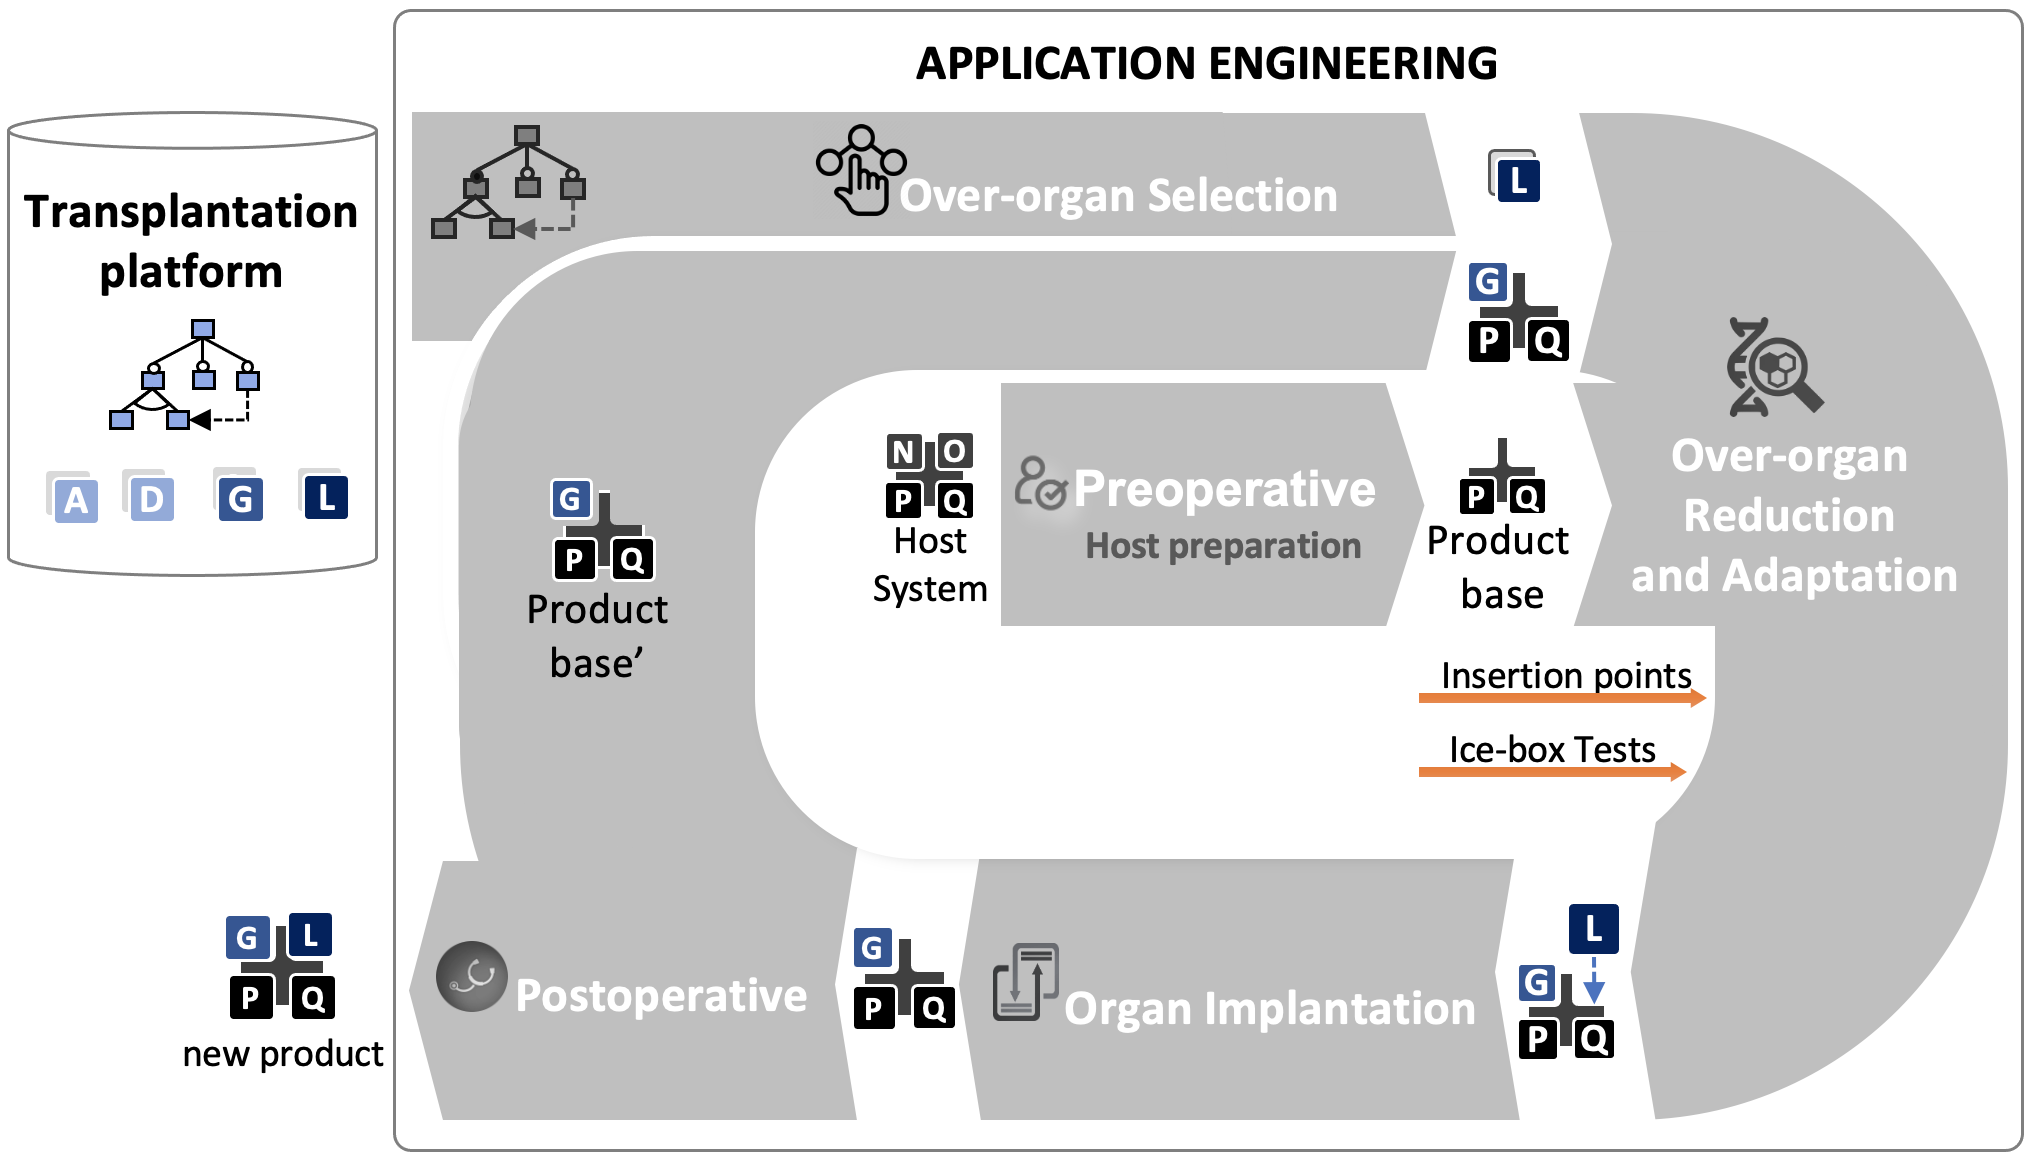
\includegraphics[width=0.9\textwidth]{images/FOUNDRY_APP5.png}
	\centering \caption{Application engineering process supported by FOUNDRY. \textit{A new product is derived after two software transplantation iterations (organs G and L).}}
	\label{fig:foundry_app}
\end{figure} 

\textbf{Over-organ Selection.} At the start of the transplantation process, an SPL engineer selects the target features that will be transplanted into the product base to create the target product. 
The choice is guided by the feature model generated during the variability analysis process, so as, to support the SPL engineer to handle eventual relationship and restrictions among transplanted organs. Once the target feature is chosen in the feature model, it is possible to find the corresponding over-organ in the transplantation platform.

\textbf{Over-organ Reduction and Adaptation.} The over-organ reduction and adaptation processes involve specialising the organ to the host environment, i.e., the product base. An SPL engineer must select the target product base with an annotated implantation point where a call to the organ will be grafted to initialize and execute it. 

Barr et al.~\cite{Barr2015} automated the over-organ reduction and adaptation process using a GP algorithm.
GP reduces an over-organ and specialises it to the host environment.
It thus creates an organ that preserves the original behaviour of the feature at a given insertion point in the host environment. 
However, Barr et al.'s approach does not support the adaptation of an organ that contains multiple files. 
Moreover, it does not support organ maintenance tasks, but rather provides a one-off transplantation approach.
To overcome these issues \FOUNDRY introduces an organ-host wrapper.
This layer is responsible for providing access to the organ from the target host. 
It is automatically constructed on demand, according to a given implantation point in the product base. 

The organ-host wrapper frees developers from the burden of manually writing the code to convert host's data structures into parameters to the organ's entry point whenever a new product is demanded from the product line.

\label{implantation}
\textbf{Organ Implantation.} In this stage of the process, the organ is ready to be implanted into the product base. 
However, to make the application of this technique in generating SPL feasible, we have to consider the transplantation of multiple organs into a single host, a product base, including ones extracted from the same donor. 
As a consequence, the process is no longer concerned with a single but multiple organs and its consequent dependency and interactions.

Feature dependency is a well-known problem in software reuse~\cite{Ribeiro2011}. Dependencies among features are established by means of structural dependencies in the source code shared between elements of different features~\cite{CafeoA2016}. In practice, an organ implementing a feature in a system often shares elements, such as variables and functions with one or more organs that belong to the same donor. For instance, a structure that stores data that are manipulated by more than one function or file; or a function call between the code that belongs to organ A and B. When this happens, the \emph{organ collision} problem occurs since both organ A and B extracted from the same donor must contain the shared function. 

\Cref{fig:organs_connection_point} shows a real-world example of two call graphs from the same donor, GEdit text editor, sharing several functions. If we consider them as part of two unrelated organs, all common functions (highlighted by blue boxes) will be duplicated during their corresponding implantation processes. As a consequence of organ collision, transplantation process can insert code that is duplicated from multiple organ transplantations. Such a problem, if it is not managed, will lead to unwanted duplicated code, possibly breaking the postoperative product. 

\begin{figure}[t]
	\centering 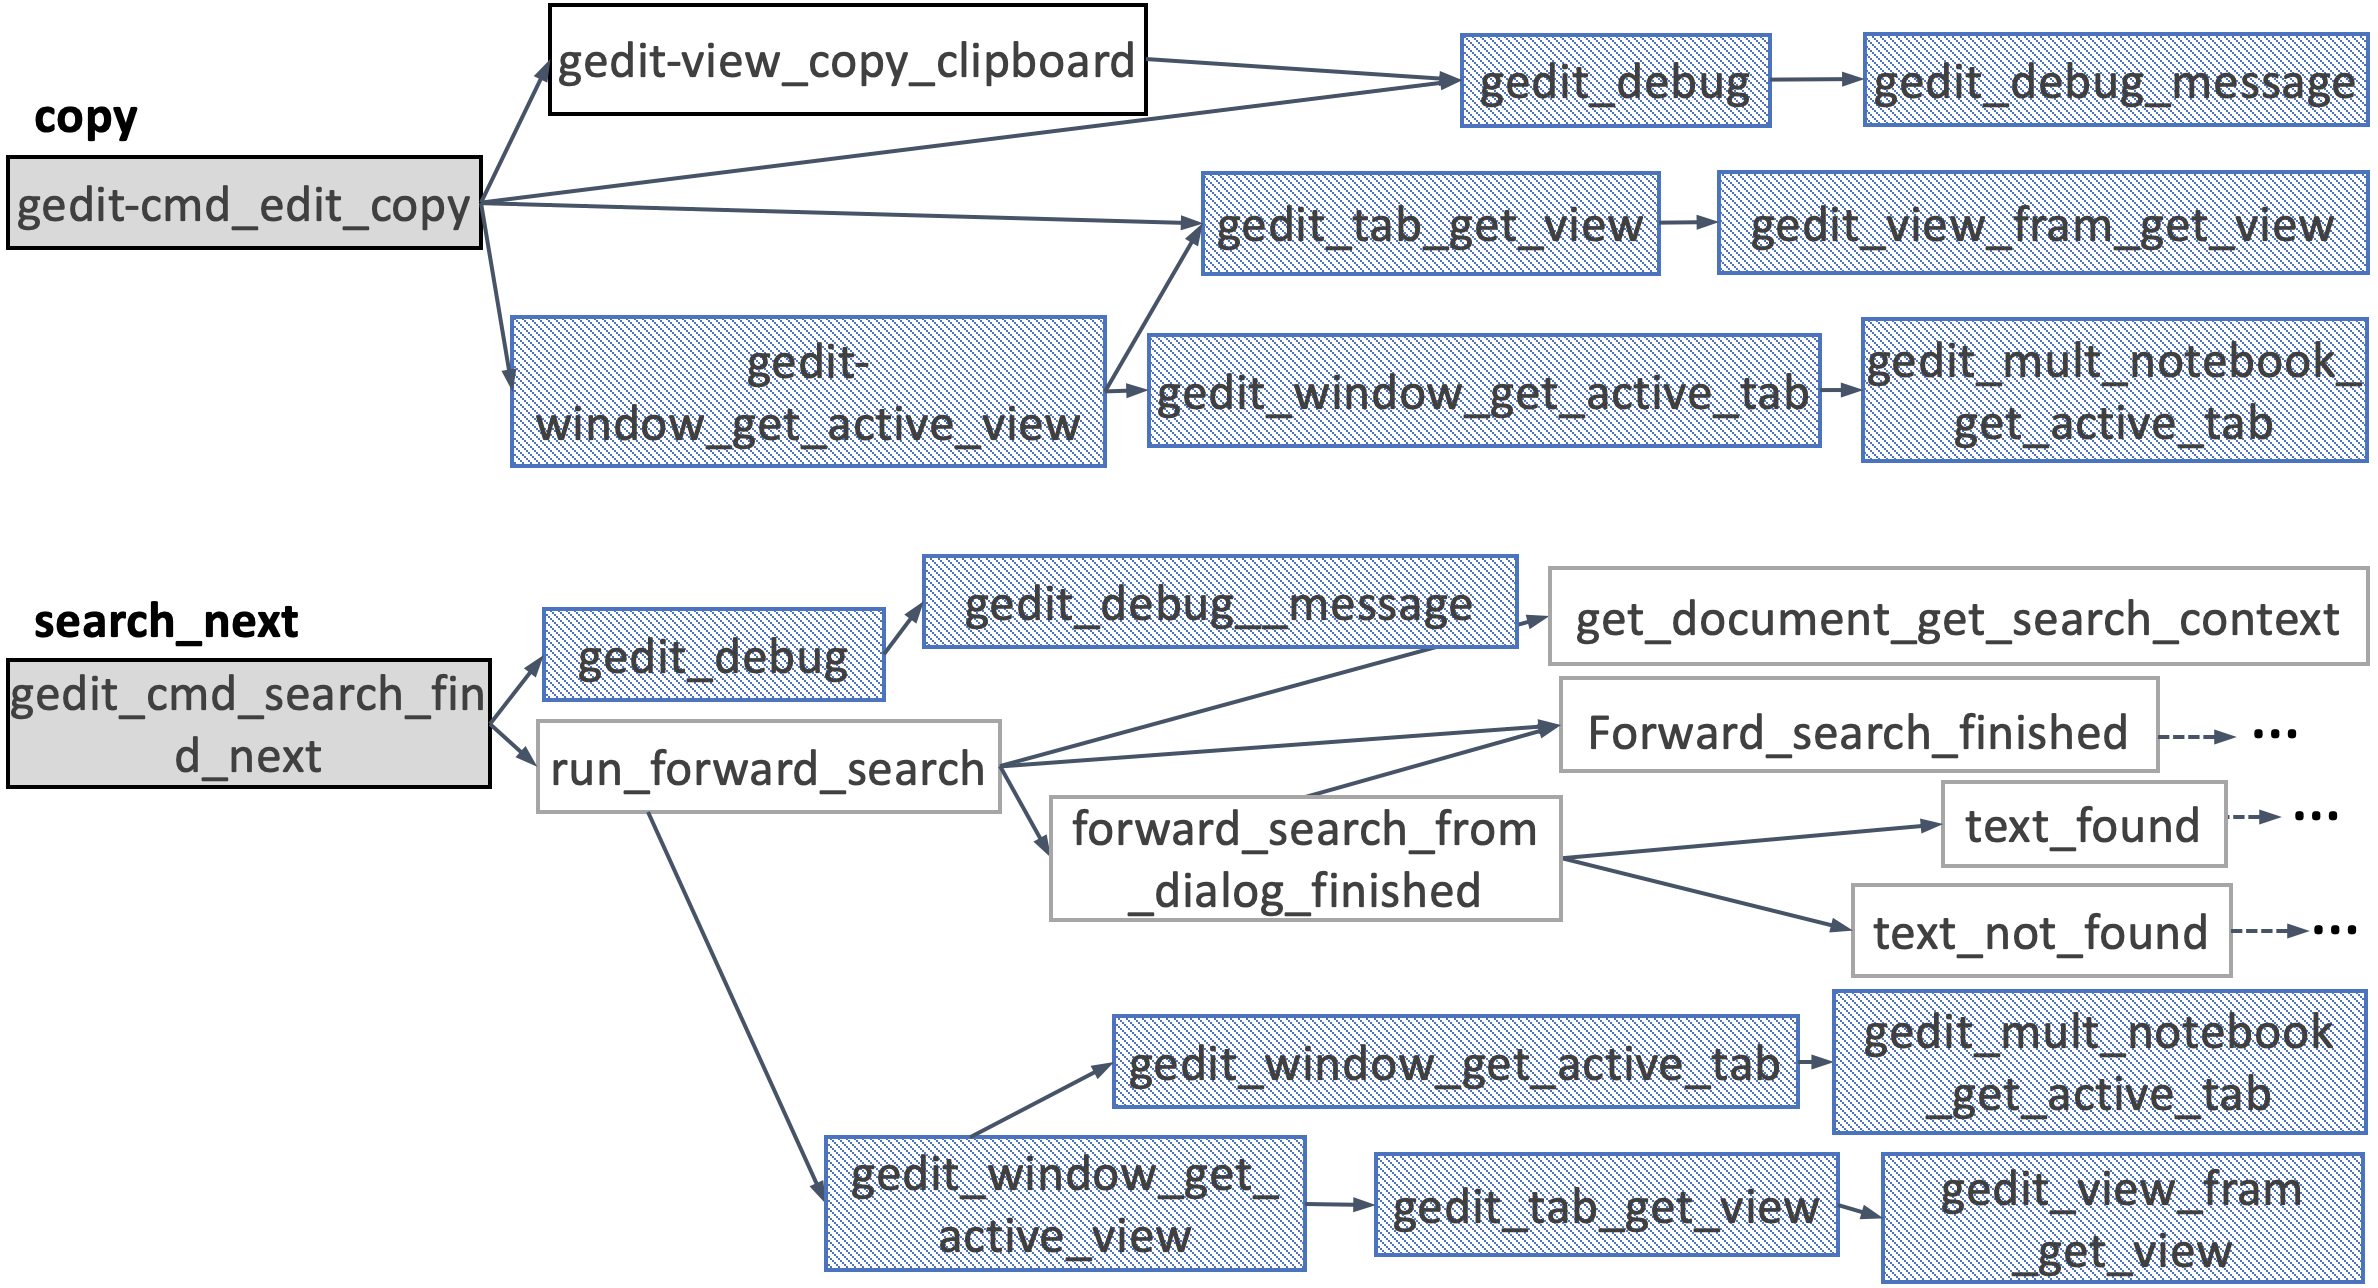
\includegraphics[width=\linewidth]{images/organs_dependency3.png}	\caption{Call graph extracted from GEdit text editor. \textit{An example of connection points among call graphs from organs $\texttt{copy}$ and $\texttt{search\_next}$. Highlighted with blue boxes are functions belonging to both organs.}}
%	\Description{The 1907 Franklin Model D roadster.}
	\label{fig:organs_connection_point}
\end{figure} 

In \FOUNDRY, code elements (functions, directives, constants, declarations of several global variables and their definitions) already belonging to the beneficiary or to more than one organ are characterized as \emph{implicit connection points} since they can represent a connection or dependence points among two or more organs. 

To correctly work, the implantation process need to identify all duplicated code elements and insert them only once into the product base, avoiding code duplication. However, hosts tend to have large input spaces into which code is inserted. In this way, finding the implicit connection points in the host can be difficult. For instance, functions can have the same namespace but not be identical. Thus, it is necessary to check whether a specific code element is already present in the host, considering not only its namespace but its structure and context at a fine level of granularity to make sure that two portions of code are "clones".

Such particular aspect represents a new challenge in the software transplantation field for SPL, handled by \FOUNDRY. 
We solve this challenge by using code clone detection, to avoid duplicated code insertion.

\textbf{Postoperative Stage.} As in medicine, \FOUNDRY requires checking the side-effects of the transplantation operation. Based on \cite{Barr2015}, \FOUNDRY's postoperative stage introduces three validation steps, as outlined in \Cref{fig:postoperative_tests}. Extending the validation process proposed in~\cite{Harman2013, Barr2015}, we highlight the three test suites that \FOUNDRY uses to evaluate the quality of a transplant: \emph{Regression}, \emph{Regression++}, and/or \emph{Acceptance} tests.
Once selected, organ has been successfully transplanted, and the postoperative product has passed all postoperative validation steps, we incorporate the Regression++ and Acceptance tests into the host's existing regression test suite for use in the next transplantation.

\begin{figure}[t]
\centering 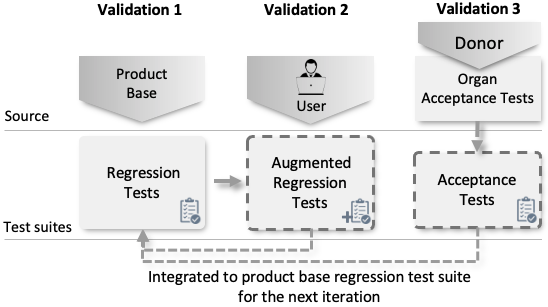
\includegraphics[width=0.6\textwidth]{images/postoperative_tests2.png}
\caption{Three validation steps; the dashed boxes are test cases added into the host regression test suite after each transplant iteration.}
\label{fig:postoperative_tests}
\end{figure} 

After the postoperative stage, new iterations of organ transplantation can be performed; thus, in a stepwise and incremental way, a new product is derived as organs are transplanted into a product base. 

